\chapter{Расчёт наилучшего транспорта передачи данных} \label{appendix:calculBestTransferDataWay}

Зададим значимость к критерия для расчётов. Количество запросов  на опрос сервера (Cnt req on poll): 4. Количество служебных заголовков вместе с ответом (Cnt of serv head): 3. Служебная информация прикрепляемая в ответе и запросе (Service info): 5. Согласно \taref{comparisonOfTypesOfDataTransmission}, модель соответствия вариантов критериям имеет следующие значения:

\begin{lstlisting}
{
	"name": "Choose transfer data",
	"criteria": { 
		"Cnt req on poll"		: 4,
		"Cnt of serv head"	: 3,
		"Service info"			: 5
	},
	"options": {
		"WebSockets"         :   [4, 4, 5],
		"Server-sent events" :   [4, 4, 4],
		"Long Polling"       :   [4, 3, 2],
		"Ajax Polling"       :   [3, 3, 2]
	} 
}
\end{lstlisting}

Расчёт наилучшего решения приведённой модели из Приложения \ref{appendix:methodSaati}:

\begin{figure}
	\centering
	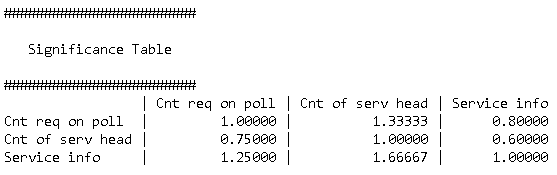
\includegraphics[width=1\linewidth]{my_folder/images/ATransferData1}
	\caption{Таблица значимости}
	\label{fig:atransferdata1}
\end{figure}

\begin{figure}
	\centering
	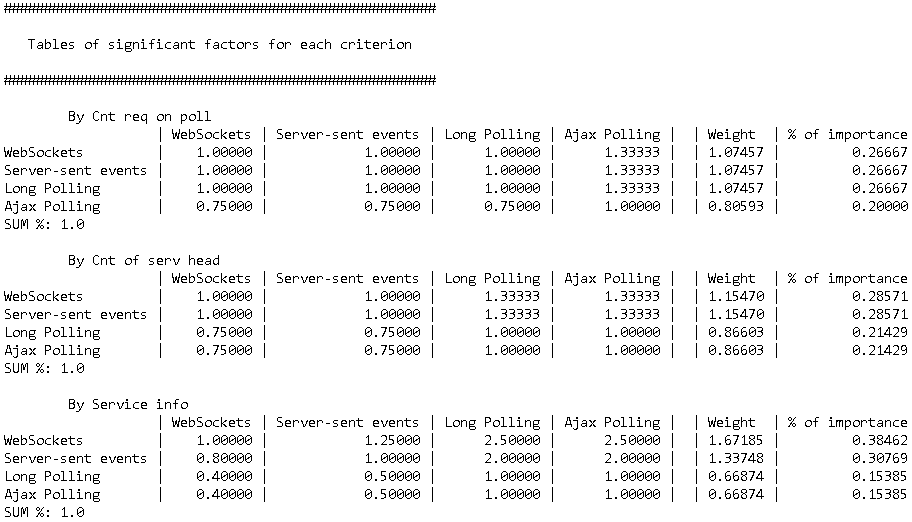
\includegraphics[scale=0.7, angle=270]{my_folder/images/ATransferData2}
	\caption{Таблицы значимых факторов для каждого критерия}
	\label{fig:atransferdata2}
\end{figure}

\begin{figure}
	\centering
	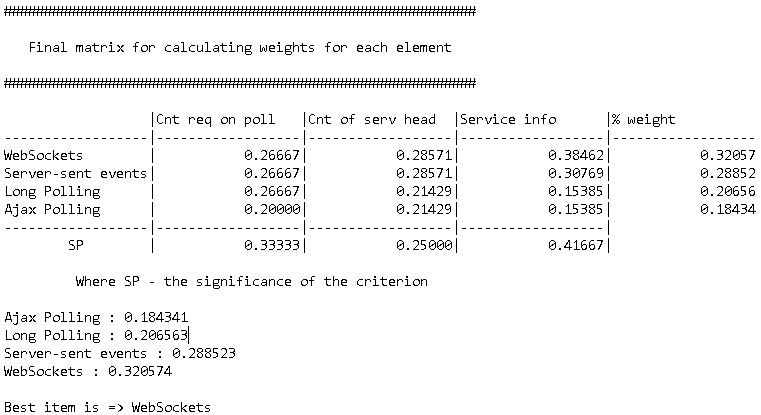
\includegraphics[width=1\linewidth]{my_folder/images/ATransferData3}
	\caption{Результируюящя таблица}
	\label{fig:atransferdata3}
\end{figure}